\documentclass{sig-alternate-05-2015}
\usepackage[utf8]{inputenc}
\usepackage{graphicx}

\begin{document}

% Copyright
\setcopyright{acmcopyright}
%\setcopyright{acmlicensed}
%\setcopyright{rightsretained}
%\setcopyright{usgov}
%\setcopyright{usgovmixed}
%\setcopyright{cagov}
%\setcopyright{cagovmixed}

\title{Procesamiento de Grafos Usando la Librería SNAP y Gephi}
%
% You need the command \numberofauthors to handle the 'placement
% and alignment' of the authors beneath the title.
%
% For aesthetic reasons, we recommend 'three authors at a time'
% i.e. three 'name/affiliation blocks' be placed beneath the title.
%
% NOTE: You are NOT restricted in how many 'rows' of
% "name/affiliations" may appear. We just ask that you restrict
% the number of 'columns' to three.
%
% Because of the available 'opening page real-estate'
% we ask you to refrain from putting more than six authors
% (two rows with three columns) beneath the article title.
% More than six makes the first-page appear very cluttered indeed.
%
% Use the \alignauthor commands to handle the names
% and affiliations for an 'aesthetic maximum' of six authors.
% Add names, affiliations, addresses for
% the seventh etc. author(s) as the argument for the
% \additionalauthors command.
% These 'additional authors' will be output/set for you
% without further effort on your part as the last section in
% the body of your article BEFORE References or any Appendices.

\numberofauthors{1} %  in this sample file, there are a *total*
% of EIGHT authors. SIX appear on the 'first-page' (for formatting
% reasons) and the remaining two appear in the \additionalauthors section.
%
\author{
% You can go ahead and credit any number of authors here,
% e.g. one 'row of three' or two rows (consisting of one row of three
% and a second row of one, two or three).
%
% The command \alignauthor (no curly braces needed) should
% precede each author name, affiliation/snail-mail address and
% e-mail address. Additionally, tag each line of
% affiliation/address with \affaddr, and tag the
% e-mail address with \email.
%
% 1st. author
\alignauthor
Alejandro Herce\\
       \affaddr{Tecnológico de Monterrey Campus Santa Fe}\\
       \affaddr{Carlos Lazo 100, Colonia Santa Fe.}\\
       \affaddr{Distrito Federal, México}\\
       \email{A01021150@itesm.mx}
}

\maketitle
\begin{abstract}
Este documento demuestra los pasos realizados en la investigación para importar un grafo de ejemplo de Stanford Large Network Dataset Collection sobre la red social Twitter, que se importará en la librería de SNAP, donde posteriormente será procesado y se exportará en diferentes formatos incluyendo GraphML, GEFX, GDF y GraphSON, basado en JSON. Posteriormente, se importarán los grafos generados en Gephi para generar la visualización de estos.

\end{abstract}


\keywords{Grafo; JSON, Gephi, GraphML, GEFX, GDF, GraphSON}

\section{Introducción}
En computación, un grafo es una estructura de datos que consiste en un conjunto de objetos llamados nodos, unidos por aristas o arcos. Un grafo típicamente se representa como un conjunto de puntos \textit{(nodos)} unidos por líneas \textit{(aristas)}. Existen dos tipos de grafos, dirigidos y no dirigidos. Los grafos dirigidos son aquellos en los que las aristas o arcos apuntan en una dirección, y en los no dirigidos las aristas apuntan en ambas direcciones.

En esta investigación, utilizamos la librería de SNAP para procesar nuestro grafo, la cual fue creada por Stanford en 2004. La librería SNAP \textit{(Stanford Network Analisis Platform)} es una librería para data mining en grafos escrita en C++ y que puede ser escalada a millones de nodos y aristas. La librería también permite manipular grafos de gran tamaño, calcular propiedades estructurales y generar grafos aleatoriamente.


\section{Trabajando con los grafos}
Como ya habíamos mencionado, utilizaremos SNAP para importar y procesar nuestro grafo, que después se exportará a cuatro diferentes formatos. La información del grafo fue obtenida del \textit{Stanford Large Network Dataset Collection}\footnote{Link: https://snap.stanford.edu/data/index.html}, en donde se pueden descargar varios datasets recolectados por Stanford sobre diferentes redes sociales. 

Nuestro dataset elegido es el de la red social Twitter, que cuenta con 81,306 nodos y 1,768,149 aristas. 


\subsection{Importando el Grafo}
Una vez seleccionado y descargado el dataset a utilizar, necesitamos importarlo a nuestro programa en donde será procesado por la librería \textit{SNAP}. El archivo del dataset es un txt en donde se incluyen todos los nodos y aristas necesarios para generar el grafo, sólo se tiene que importar con nuestra librería. El archivo txt se tiene que ubicar en el mismo folder que nuestro main.cpp para que pueda ser leído por \textit{SNAP}.

Después de inicializar un grafo en \textit{SNAP}, tenemos que importar los datos del archivo txt. Para importar el dataset, sólo se requiere una línea de código: 

\textit{TSnap::LoadEdgeList<Graph>("twitter.txt",0,1);}


\subsection{Procesando y Exportando el Grafo}
Como habíamos mencionado, el grafo se exportará en cuatro diferentes formatos, GraphML, GEFX, GDF y JSON a través de la librería GraphSON. No tocaremos los detalles específicos de cada formato, pues la documentación es accesible para todos.

De forma muy general, al exportar nuestro grafo en realidad lo que estamos haciendo es guardar los nodos y aristas como si fuera un documento txt pero con una plantilla especifica para cada librería. Por ejemplo, los nodos en GraphML se guardan así: \textit{<node id=”nodo1”>} y de la misma forma las aristas. Las librerías no son iguales, pero lo que importa es el concepto de la plantilla, que es muy parecido a hacer una lista de nodos y aristas, solo que con mas símbolos.

Para exportar el grafo, lo único que se tiene que hacer es un ciclo \textit{for} donde se va recorriendo el grafo nodo por nodo y arista por arista y guardándolo en el archivo con la plantilla correspondiente al formato seleccionado.

\subsection{Tiempos de Ejecución}
Además de exportar el grafo, el programa también mide el tiempo de ejecución al exportar en cada formato. El tiempo se mide con la función \textit{high resolution clock}, tomando el tiempo justo antes de la ejecución y justo al terminar para después hacer una resta y obtener el tiempo en milisegundos que tardó en ejecutarse cada función de exportación. 

Para ejecutar el programa, se utilizó una maquina virtual de Ubuntu con 4 GB de RAM y 4 cores (2 reales y 2 en hyperthreading). Los tiempos para exportar 81,306 nodos y 1,768,149 aristas a los cuatro formatos se pueden apreciar en la Tabla 1.

\begin{table}
\centering
\caption{Tiempos de ejecución}
\begin{tabular}{|c|c|} \hline
Función&Tiempo (Milisegundos)\\ \hline
GraphML & 775\\ \hline
GEFX & 1536\\ \hline
GDF & 677\\ \hline
GraphSON & 1330\\
\hline\end{tabular}
\end{table}


\subsection{Importando en Gephi}
Una vez exportado el grafo en los diferentes formatos, podemos importarlo en Gephi. Gephi es un programa multi plataforma para la visualización y exploración interactiva de todo tipo de redes y sistemas complejos, como grafos. Gephi permite importar, explorar y manipular grafos en tiempo real, además de poder exportarlos en varios formatos como PDF y PNG. Este programa es compatible con tres formatos en los que exportamos nuestro grafo: GraphML, GEFX y GDF.

Una vez importado el grafo en Gephi, se le aplicaron colores a los nodos en varios tonos de azul al blanco y después se le aplico la función Force Atlas 2. Dicha función es un algoritmo continuo para la espacialización de redes que funciona aplicando fuerzas, repeliendo los nodos unos de otros como imanes, pero al mismo tiempo las aristas actúan como resortes uniéndolos. Estas fuerzas crean un balance, lo que permite que el resultado final sea mas comprensible.

Los resultados del algoritmo aplicado al grafo se pueden ver en las Figuras 1 y 2.


\section{Conclusiones}
El proceso de importar y exportar el grafo en diferentes formatos fue relativamente simple. Es un simple archivo en el cual se inserta una lista de nodos y aristas. Los problemas surgieron cuando pasamos a la parte de Gephi, pues el programa es un poco lento y con la cantidad de nodos y aristas generados tardó mucho en importar y en aplicar el algoritmo Force Atlas 2. 

Originalmente quería usar el dataset de Youtube con mas de 1 millón de nodos y casi 3 millones de aristas, pero Gephi no se dejó y se cerro varias veces. En la parte de exportarlo a los cuatro formatos, no tuve ningún problema y los tiempos de ejecución rondaban entre los mil y dos mil milisegundos, bastante decentes si consideramos el tamaño del grafo.

En general el proceso fue muy simple y Gephi ofrece muchas opciones para explorar los grafos, pero faltó un poco mas de tiempo para aprender un poco mas acerca de este programa.


\section{GitHub}
https://github.com/alexherce/Algoritmos

\begin{figure}
\centering

\includegraphics[height=4in, width=4in]{gephibefore}
\caption{Antes de Force Atlas 2}
\end{figure}

\begin{figure}
\centering
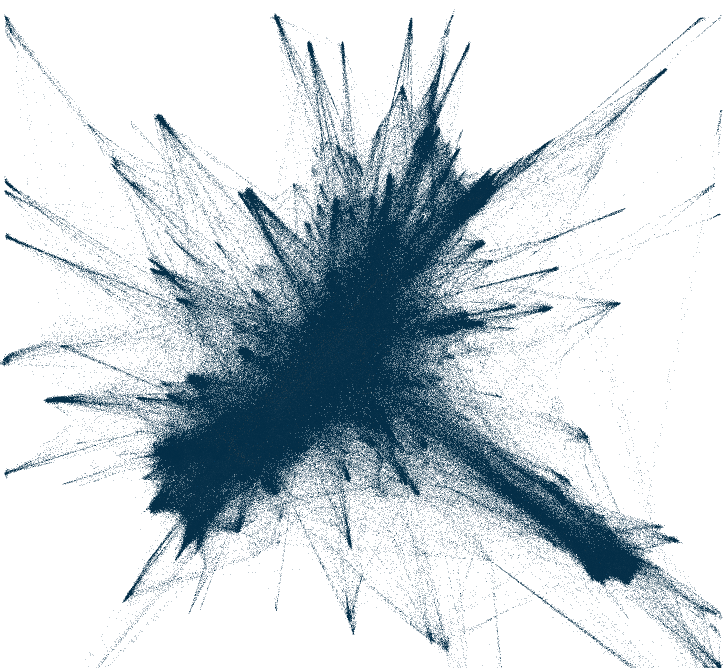
\includegraphics[height=4in, width=4in]{gephiafter}
\caption{Después de Force Atlas 2}
\end{figure}

\end{document}
